\documentclass[12pt,letter]{article}

%% \ifCLASSOPTIONcompsoc
%% % IEEE Computer Society needs nocompress option
%% % requires cite.sty v4.0 or later (November 2003)
%% \usepackage[nocompress]{cite}
%% \else
%% % normal IEEE
%% \usepackage{cite}
%% \fi

%% \usepackage[fleqn]{amsmath}
\usepackage[margin=1.0in]{geometry}
\usepackage{amsmath,amsfonts,amsthm,bm}
\usepackage{breqn}
\usepackage{amsmath}
\usepackage{amssymb}
\usepackage{tikz}
\usepackage{algorithm2e}
\usepackage{siunitx}
\usepackage{graphicx}
\usepackage{subcaption}
%% \usepackage{datetime}
\usepackage{multirow}
\usepackage{multicol}
\usepackage{mathrsfs}
\usepackage{fancyhdr}
\usepackage{fancyvrb}

\pagestyle{fancy}

\usetikzlibrary{arrows}

\DeclareMathOperator*{\argmin}{argmin}
\newcommand*{\argminl}{\argmin\limits}

\newcommand{\mathleft}{\@fleqntrue\@mathmargin0pt}
\newcommand{\R}{\mathbb{R}}
\newcommand{\Z}{\mathbb{Z}}
\newcommand{\N}{\mathbb{N}}

\begin {document}

\rhead{(Bill) Yuan Liu, student \#: 996954078\\ Date: 2019/11/22}
\lhead{ECE1647F - Nonlinear Systems - Assignment 4}

\begin{itemize}
  
\item 3.8\\
  \begin{align*}
    \text{let } \tilde{x}&=x-\hat{x}\\
    \dot{\tilde{x}}&=Ax+f(x)-(A\hat{x}+f(\hat{x})+L(y-C\hat{x})\\
                         &=(A-LC)\tilde{x}+f(x)-f(\hat{x})\\
    \text{Desired property of observer: } & lim_{t \to \infty}\tilde{x}(t)=0\\
    \text{let } V(\tilde{x})&=\tilde{x}^TP\tilde{x}\\
    V(\tilde{x}^*=0)&=0\\
    \text{using theorem 3.24:}\\
    \forall\sigma(A-LC)<0 & \implies (\exists P,Q) P(A-LC)+(A-LC)^TP=-Q,\\ & \text{where } Q,P \text{ are spd}\\
                         & \implies V(\tilde{x}) \text{ is a pd function}\\
    \text{using Lyapunov direct method: }\\
    L_{\dot{\tilde{x}}}V(\tilde{x}) & < 0 \text{ at } \tilde{x}^*\\
    L_{\dot{\tilde{x}}}V(\tilde{x}) & = 2\tilde{x}^TP((A-LC)\tilde{x}+f(x)-f(\tilde{x}))\\
    L_{\dot{\tilde{x}}}V(\tilde{x}) & = -\tilde{x}^TQ\tilde{x} + 2\tilde{x}^TP(f(x)-f(\hat{x}))<0\\
    2\tilde{x}^TP(f(x)-f(\hat{x})) & < \tilde{x}^TQ\tilde{x}\\
    \|2\tilde{x}^TP(f(x)-f(\hat{x}))\| & < \|\tilde{x}^TQ\tilde{x}\|\\
    \|2\tilde{x}^TP(f(x)-f(\hat{x}))\| & \leq 2\|\tilde{x}^T\|\|P\| K \|\tilde{x}\| < \tilde{x}^TQ\tilde{x}\\
    K & < \frac{\tilde{x}^TQ\tilde{x}}{2\|\tilde{x}^T\|\|P\| \|\tilde{x}\|}\\
    \text{if }Q=I, Q \text{ is Hermitian,} \text{ use Rayleigh Quotient}:\\
    1=\lambda_{min}(I) \leq & \frac{x^TQx}{x^Tx} \leq \lambda_{max}(I)=1\\
    K & < \frac{\|\tilde{x}\|_2^2}{2\|\tilde{x}^T\|\|P\| \|\tilde{x}\|}\\
    \|*\|_2 & = $ spectral radius$(*)\\
    K & < \frac{1}{2\|P\|_2}=\frac{1}{2\ \lambda_{max}(P)}\\
  \end{align*}
  This gives the bound on f's Lipschitz constant with chosen $Q,P$ of the Lyapunov function.\\
  
  With $V$ positive definite and $L_{\dot{\tilde{x}}}V(\tilde{x})$ negative definite at $\tilde{x}^*$, $\tilde{x}^*$ is an asymptotically stable equilibrium so an observer $\dot{\hat{x}}=A\hat{x}+f(\hat{x})+L(y-C\hat{x})$ exists.

  \pagebreak
  
\item 3.9\\
  $f=\dot{x}=Ax+g(x)$, $\|g(x)\| \leq \gamma \|x\|_2^2$, $g$ is locally Lipschitz\\
  \begin{enumerate}
    \item prove exponentially stable equilibrium exists at the origin\\
      
      use Lyapunov indirect method:\\
      $lim_{\|x\| \to x^*=0} \frac{\|f(x)-f(0)-dfx\|}{\|x\|}=0$\\
      $f(0)=A0+g(0)=0$\\
      linearization near $x^*=0$ with Taylor expansion:\\
      $f(x \text{ near 0}) \approx A0 + g(0) + A + \dot{g}|_{x=0}=A+(O(\gamma \|x\|_2^2)I)|_{x=0} = A$\\
      $df|_{x=0}=A$\\
      $\forall \sigma(A) < 0 \implies \text{ linearization }\dot{x} = df|_{x=0} x$ is asymptotically stable, then $x^*=0$ is an exponentially stable equilibrium of $f$.\\

    \item estimate domain of attraction\\

      from part 1, $df_{x^*}$ is Hurwitz\\
      pick a spd Q=I, solve spd P for Lyapunov equation $PA+A^TP=-Q$\\
      let $V(x)=x^TPx$\\
      $\frac{\partial V}{\partial t} = (\frac{\partial V}{\partial (x-x^*)})(\frac{\partial}{t} (x-x^*))$\\
      near $x^*$:\\
      let $\tilde{x}=x-x^*$\\
      $\frac{\partial V}{\partial t} = ((P\tilde{x})^T+\tilde{x}^TP)(df_{x^*}+f(x)-df_{x^*}\tilde{x})$\\
      $\frac{\partial V}{\partial t} = (\tilde{x}^TPdf_{x^*}+\tilde{x}^TPdf_{x^*})+2\tilde{x}^TP(f(x)-df_{x^*}\tilde{x})$\\
      $\frac{\partial V}{\partial t} = (\tilde{x}^TPA\tilde{x}+(\tilde{x}^TPA\tilde{x})^T)+2\tilde{x}^TP(f(x)-df_{x^*}\tilde{x})$\\
      $\frac{\partial V}{\partial t} = -\tilde{x}^TQ\tilde{x}+2\tilde{x}^TP(f(x)-df_{x^*}\tilde{x})$\\
      $\frac{\partial V}{\partial t} = -x^TQx+2x^TP(Ax+g(x)-(A(x-0)))$\\
      $\frac{\partial V}{\partial t} = -x^TQx+2x^TPg(x)$\\
      let $D=\{x: - x^TQx+2x^TPg(x) \leq 0 \}$ be connected and $0 \in D$\\
      $Q=I$ is Hermitian $\implies$ $\lambda_{min}(Q) \leq \frac{x^TQx}{x^Tx} \leq \lambda_{max}(Q)$\\
      $\frac{x^TQx}{x^Tx}=1$, $x^TQx=x^Tx$\\
      $- x^Tx + 2x^TPg(x) \leq 0 $\\
      $- x^Tx + 2x^TPg(x) \leq - x^Tx + 2\|x^TP\|\gamma\|x\|_2^2 \leq 0 $\\
      $-1 + 2\|x\|_2\|P\|_2\gamma \leq 0 $\\
      $\|x\|_2 \leq \frac{1}{2 \gamma \|P\|_2}$\\
      $D=\{x: \|x\|_2 \leq \frac{1}{2 \gamma \|P\|_2} \}$\\
      let $c^*=inf_{x \in \partial D}\{ (x-0)^TP(x-0) \}$\\
      $\lambda_{min}(P)  x^Tx \leq x^TPx \leq \lambda_{max}(P) x^Tx, \|x\|_2 \leq \frac{1}{2 \gamma \|P\|_2}$\\
      $\lambda_{min}(P)  x^Tx, \|x\|_2 = \frac{1}{2 \gamma \|P\|_2}, x^Tx = \|x\|_2^2 \implies \lambda_{min}(P)  x^Tx = \frac{\lambda_{min}(P)}{4\gamma^2 \lambda_{max}(P)^2}$\\
      $c^*=\frac{\lambda_{min}(P)}{4\gamma^2 \lambda_{max}(P)^2}$\\
      domain of attraction estimate: $D_{x^*}=\{x: x^TPx< c^*\}$\\
      
    \item consider:\\
      let $n=2$\\
      $A=\begin{bmatrix}0 & 1 \\ -1 & -2\end{bmatrix}$\\
      $g(x)=\begin{bmatrix}x_1^2+x_2^2 \\ 0 \end{bmatrix}$\\

      let $Q=I$\\
      $PA+A^T=-Q$\\
      $P=\begin{bmatrix}3/2 & 1/2 \\ 1/2 & 1/2 \end{bmatrix}$\\
      
      calculate $\gamma$:\\
      $\|g(x)\|_2=((x_1^2+x_2^2)^2+0^2)^{0.5}=x_1^2+x_2^2$\\
      $\|x\|_2=(x_1^2+x_2^2)^{0.5}$\\
      $\|g(x)\|_2 \leq \gamma \|x\|_2^2$\\
      $x_1^2+x_2^2 \leq \gamma ((x_1^2+x_2^2)^{0.5})^2$\\
      $x_1^2+x_2^2 \leq \gamma (x_1^2+x_2^2)$\\
      $\gamma=1$\\

      $c^*=\frac{\lambda_{min}(P)}{4\gamma^2 \lambda_{max}(P)^2}$\\
      $c^*=\frac{\lambda_{min}(P)}{4 \lambda_{max}(P)^2}=\frac{0.2929}{4(1.7071)^2}=0.0251$\\
      domain of attraction estimate: $D_{x^*}=\{x: x^TPx< 0.0251\}$
      \begin{figure}[h]
        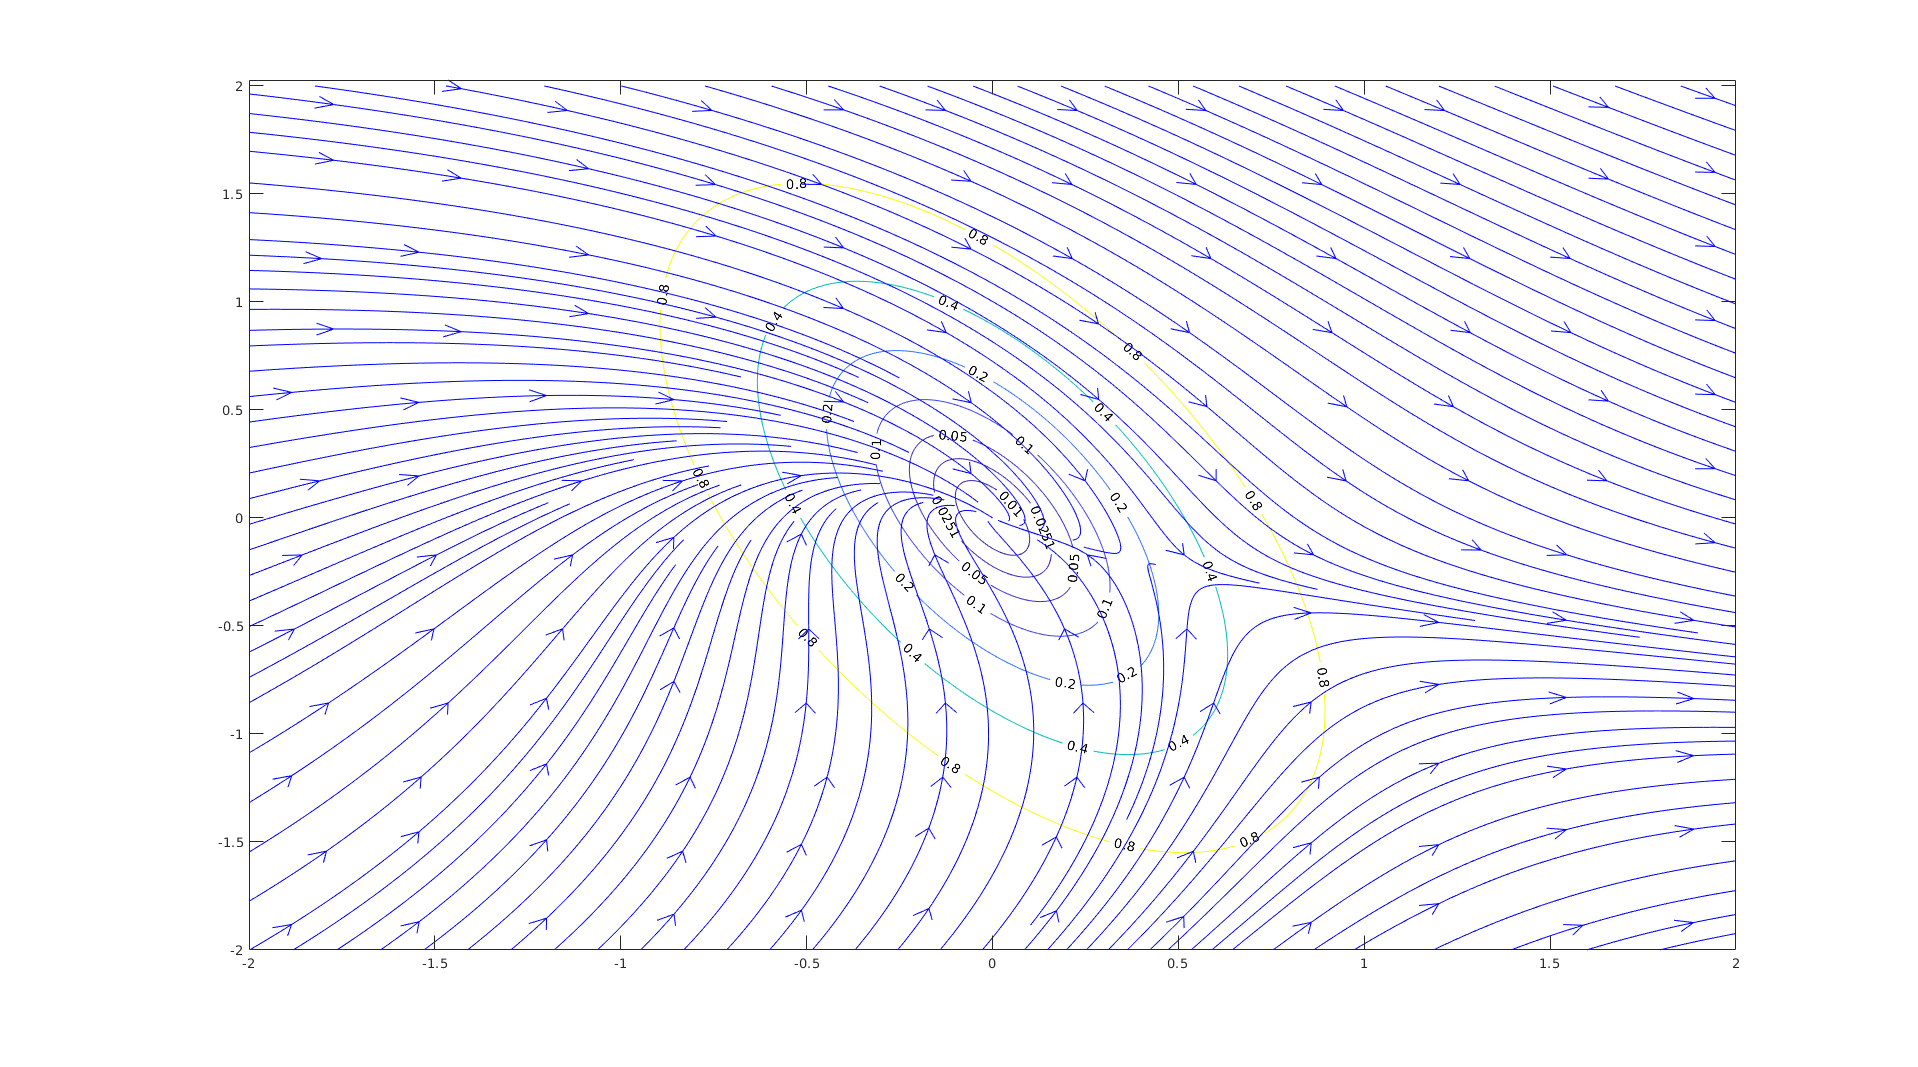
\includegraphics[width=15cm,keepaspectratio]{matlab/pics/q3_9_phase_portrait.png}
      \end{figure}\\
      From phase portrait, the estimate is conservative as it does not include a large region to the bottom left that are attractived to the origin.\\
    \end{enumerate}

    \pagebreak
    
\item 3.10\\

  $x=\begin{bmatrix}
    x_1-\pi\\
    x_2\\
    \hat{\theta}-\theta
  \end{bmatrix}$\\

  $V=
  \begin{bmatrix}
    x_1-\pi & x_2 & \hat{\theta}-\theta
  \end{bmatrix}
  P
  \begin{bmatrix}
    x_1-\pi \\ x_2 \\ \hat{\theta}-\theta
  \end{bmatrix}$\\

  $P=\begin{bmatrix}
    p_1 & p_2 & 0\\
    p_2 & p_3 & 0\\
    0 & 0 & 1/2
  \end{bmatrix}$\\
  
  $\frac{\partial V}{\partial x} =
  \begin{bmatrix}
    2p_1(x_1-\pi)+2x_2p_2\\
    2p_2(x_1-\pi)+2x_2p_3\\
    \hat{\theta}-\theta
  \end{bmatrix}$\\

  $\frac{\partial x}{\partial t} =
  \begin{bmatrix}
    x_2\\
    -c_1(x_1-\pi)-c_2x_2+(\hat{\theta}-\theta)sin(x_1)\\
    \varphi(x_1,x_2)
  \end{bmatrix}$\\

  $c_1,c_2>0$\\
  
  $L_fV = 2p_1(x_1-\pi)x_2+2p_2x_2^2+(2p_2(x_1-\pi)+2p_3x_2)((\hat{\theta}-\theta)sin(x_1)-c_1(x_1-\pi)-c_2x_2) + (\hat{\theta}-\theta)\varphi(x_1,x_2)$\\

  let $\varphi(x_1,x_2)=-(2p_2(x_1-\pi)+2p_3x_2)sin(x_1)$\\

  make $L_fV$ to be negative semidefinite at
  $x=\begin{bmatrix}
    \pi\\
    0\\
    *
  \end{bmatrix}$:\\

  $L_fV = -2p_2c_1(x_1-\pi)^2+x^2(2p_2-2p_3c_2)+x_2(x_1-\pi)(2p_1-2p_2c_2-2p_3c_1) \leq 0$\\
  $p_2 \geq 0$\\
  $p_2 - p_3c_2 \leq 0$\\
  $p_1-p_2c_2-p_3c_1=0$\\

  let $p_2=1$\\
  $p_3 \geq 1/c_2$\\
  let $p_3=2/c_2$\\
  $p_1=c_2+\frac{2c_1}{c_2}$\\

  $V=
  \begin{bmatrix}
    x_1-\pi & x_2 & \hat{\theta}-\theta
  \end{bmatrix}
  \begin{bmatrix}
    c_2+\frac{2c_1}{c_2} & 1 & 0\\
    1 & \frac{2}{c_2} & 0\\
    0 & 0 & 1/2\\
  \end{bmatrix}
  \begin{bmatrix}
    x_1-\pi \\ x_2 \\ \hat{\theta}-\theta
  \end{bmatrix}
  $

  let diagonal entries be big enough to dominate other entries in each row so that all eigenvalues are positive by Gersgorin Circle theorem: $c_1=\frac{1}{2}, c_2=1$\\
  
  $P=
  \begin{bmatrix}
    2 & 1 & 0\\
    1 & 2 & 0\\
    0 & 0 & 1/2\\
  \end{bmatrix}
  $

  $P$ is symmetric and all eigenvalues are positive so $P$ is spd.\\

  $P$ is spd, so $V$ is positive definite at 
  $\begin{bmatrix}
    \pi \\ 0 \\ \theta
  \end{bmatrix}$\\

  $sin(x_1)$ is $C^1$ and rest of terms in $\frac{\partial x}{\partial t}$ are linear and so $f$ is locally Lipschitz\\

  $V$ is a quadratic and differentiates to a linear function and is $C^1$\\

  With chosen constants, $L_fV$ is negative semidefinite at $\begin{bmatrix}
    \pi \\ 0 \\ \theta
  \end{bmatrix}$\\
  \\
  By Lyapunov direct method, $\begin{bmatrix}
    \pi \\ 0 \\ \theta
  \end{bmatrix}$ is a stable equilibrium, so all trajectories are bounded.\\

  From earlier, $L_fV = 0$ for
  $\begin{bmatrix}
    \pi \\ 0 \\ *
  \end{bmatrix}$ so the straight line at $x_1=\pi, x_2=0$ is an invariant set.\\
  
  Substituting any of these values into $f$ gives equilibrium for the original system, so the line at $x_1=\pi, x_2=0$ is a set of equilibria for the closed loop system.\\

  $\Omega=\{x: x_1=\pi, x_2=0\}$ is the largest invariant subset of the level set for $L_fV=0$, since $L_fV \leq 0$, then all solutions approaches $\Omega$ as $t \to \infty$.

  $u=ml^2(-c_1(x_1-\pi)-c_2x_2+\hat{\theta}sin(x_1))=ml^2(-1/2(x_1-\pi)-x_2+\hat{\theta}sin(x_1))$\\

  $\frac{\partial x}{\partial t} =
  \begin{bmatrix}
    x_2\\
    -\theta sin(x_1)+\frac{1}{ml^2}u\\
    -(2p_2(x_1-\pi)+2p_3x_2)sin(x_1)
  \end{bmatrix}=
  \begin{bmatrix}
    x_2\\
    -\theta sin(x_1)-1/2(x_1-\pi)-x_2+\hat{\theta}sin(x_1)\\
    -(2(x_1-\pi)+4x_2)sin(x_1)
  \end{bmatrix}
  $\\
  
  \pagebreak

\begin{verbatim}
function dx = ss_prob3(t,x)
    theta = 1;
    dx1 = x(2);
    dx2 = -theta*sin(x(1))-1/2*(x(1)-pi)-x(2)+x(3)*sin(x(1));
    dx3 = -(2*(x(1)-pi)+2*2*x(2))*sin(x(1));
    dx = [dx1; dx2; dx3];
end
t=[0 500];
ini_cond= ... ;
[~,X]=ode45(@ss_prob3,t,ini_cond);
u = X(:,1);
v = X(:,2);
w = X(:,3);
plot3(u,v,w);
\end{verbatim}
  $\theta=1, x_0=[5,5,5], [20,20,20], [50,-10,5]:$\\
  \begin{figure}[h]
    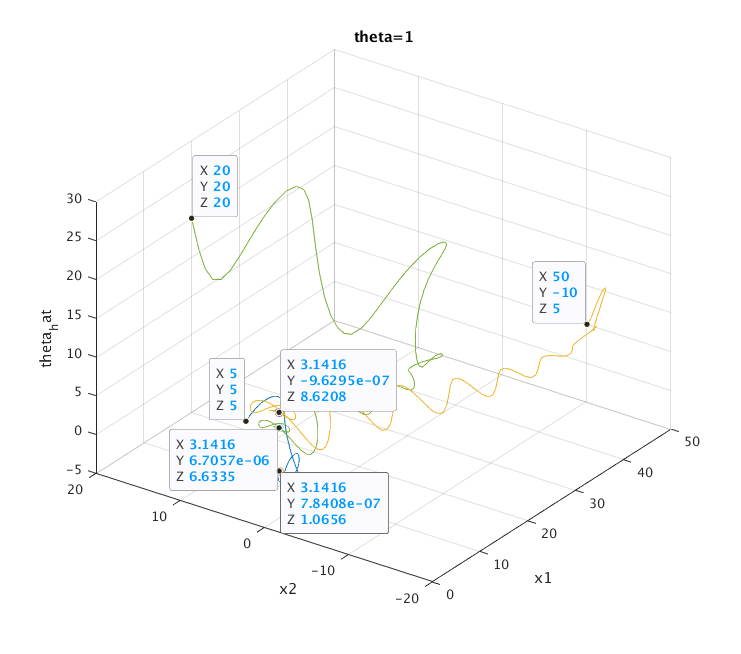
\includegraphics[width=15cm,keepaspectratio]{matlab/3_10/q3_10_theta_1.png}
  \end{figure}\\

  \pagebreak
  $\theta=-10, x_0=[5,5,5], [50,-10,5], [-30,20,20]:$\\
  \begin{figure}[h]
    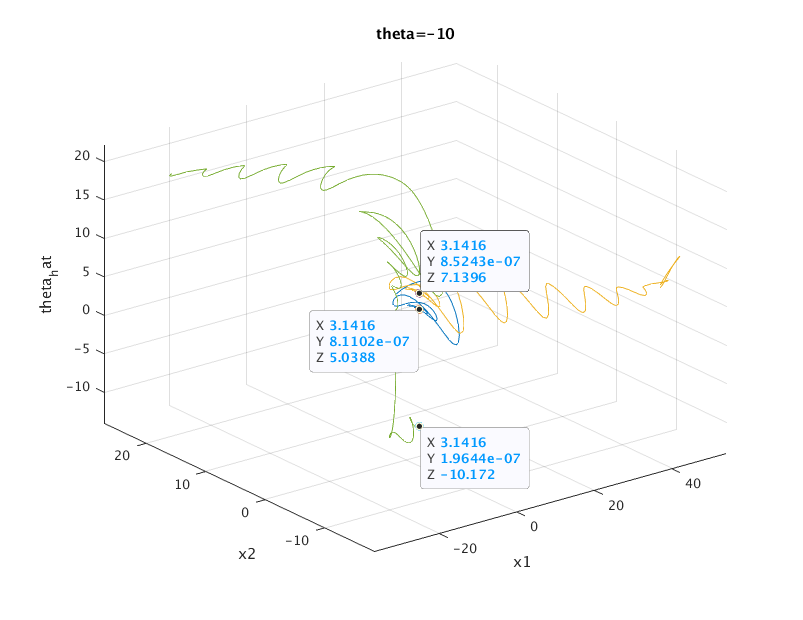
\includegraphics[width=16cm,keepaspectratio]{matlab/3_10/q3_10_theta_minus_10.png}
  \end{figure}
  
  From the plot, $x_1 \to \pi, x_2 \to 0, \hat{\theta} - \theta \not\to 0$\\
  
  \pagebreak

\item 3.11\\

$V=x^TPx$\\
  
$x=
\begin{bmatrix}
  x_1 - \pi\\
  x_2\\
  \hat{a_1}-a_1\\
  \hat{a_2}-a_2\\
\end{bmatrix}
$\\

$
\frac{\partial x}{\partial t}=
\begin{bmatrix}
  x_2\\
  sin(x_1)(\theta_2 \hat{a_1}-\theta_1)-\theta_2 \hat{a_2}\\
  c_1(x_1-\pi)+c_2 x_2\\
  \varphi_1\\
  \varphi_2\\
\end{bmatrix}
$\\

$P=
\begin{bmatrix}
  p_1 & p_2 & 0 & 0 \\
  p_2 & p_3 & 0 & 0 \\
  0 & 0 & \frac{\theta}{2} & 0\\
  0 & 0 & 0 & \frac{\theta}{2}\\
\end{bmatrix}
$\\

$a_1 = \frac{\theta_1}{\theta_2}$\\
$a_2 = \frac{1}{\theta_2}$\\
$\theta_2>0$\\

$
  \frac{\partial V}{\partial t}=
  2\begin{bmatrix}
    (x_1-\pi)p_1+p_2x_2 \\
    (x_1-\pi)p_2+p_3x_2 \\
    \theta_2(\hat{a_1}-a_1) \\
    \theta_2(\hat{a_2}-a_2)
  \end{bmatrix}^T
  \begin{bmatrix}
    x_2\\
    sin(x_1)(\theta_2 \hat{a_1}-\theta_1)-\theta_2 \hat{a_2}\\
    c_1(x_1-\pi)+c_2 x_2\\
    \varphi_1\\
    \varphi_2\\
  \end{bmatrix}
  \leq 0
$\\  

\begin{align*}
\frac{\partial V}{\partial t}=& 2( x_2^2 p_2+\\
                              & x_2(x_1-\pi)p_1+\\
                              & sin(x_1)\theta_2 \hat{a_1} (x_1 -\pi) p_2 +\\
                              & sin(x_1)(-\theta_1)(x_1-\pi)p_2 +\\
                              & sin(x_1)(\theta_2 \hat{a_1}) p_3 x_2 +\\
                              & sin(x_1)(-\theta_1) p_3 x_2 +\\
                              & \theta_2(\hat{a_1}-a_1) \varphi_1 + \theta_2(\hat{a}_2-a_2) \varphi_2\\
                              & -\theta_2 \hat{a_2}((x_1-\pi)^2 c_1 p_2 + c_2 p_3 x_2^2 + x_2(x_1-\pi)(c_2p_2 + c_1p_3))) \leq 0\\ 
\end{align*}

\pagebreak

let $\varphi_2 = (x_1-\pi)^2c_1 p_2 + c_2 p_3 x_2^2 + x_2(x_1 -\pi)(c_2 p_2 + c_1 p_3)$\\

$\theta_2 a_2 = 1$\\

$
\theta_2(\hat{a}_2-a_2) \varphi_2 -\theta_2 \hat{a_2}((x_1-\pi)^2 c_1 p_2 + c_2 p_3 x_2^2 + x_2(x_1-\pi)(c_2p_2 + c_1p_3))\\
=\theta_2 \hat{a_2}((x_1-\pi)^2 c_1 p_2 + c_2 p_3 x_2^2 + x_2(x_1-\pi)(c_2p_2 + c_1p_3))\\
-\theta_2 \hat{a_2}((x_1-\pi)^2 c_1 p_2 + c_2 p_3 x_2^2 + x_2(x_1-\pi)(c_2p_2 + c_1p_3))\\
-\theta_2 a_2((x_1-\pi)^2 c_1 p_2 + c_2 p_3 x_2^2 + x_2(x_1-\pi)(c_2p_2 + c_1p_3))\\
=-((x_1-\pi)^2 c_1 p_2 + c_2 p_3 x_2^2 + x_2(x_1-\pi)(c_2p_2 + c_1p_3))\\
$\\

let $\varphi_1 = -sin(x_1)((x_1-\pi) p_2 + p_3 x_2)$\\
$\theta_2 a_1 = \theta_2 \frac{\theta_1}{\theta_2}=\theta_1$\\

$\theta_2(\hat{a_1}-a_1) \varphi_1\\
=(\theta_2\hat{a_1}-\theta_1) \varphi_1\\
=-sin(x_1)(\theta_2 \hat{a_1})((x_1-\pi) p_2 + p_3 x_2) +
sin(x_1)(\theta_1)((x_1-\pi) p_2 + p_3 x_2)\\
$\\

$
sin(x_1)\theta_2 \hat{a_1} (x_1 -\pi) p_2 +\\
sin(x_1)(-\theta_1)(x_1-\pi)p_2 +\\
sin(x_1)(\theta_2 \hat{a_1}) p_3 x_2 +\\
sin(x_1)(-\theta_1) p_3 x_2 +\\
+\theta_2(\hat{a_1}-a_1) \varphi_1\\
=0\\
$\\

Then,

$
x_2^2 p_2+\\
& x_2(x_1-\pi)p_1+\\
& sin(x_1)\theta_2 \hat{a_1} (x_1 -\pi) p_2 +\\
& sin(x_1)(-\theta_1)(x_1-\pi)p_2 +\\
& sin(x_1)(\theta_2 \hat{a_1}) p_3 x_2 +\\
& sin(x_1)(-\theta_1) p_3 x_2 +\\
& \theta_2(\hat{a_1}-a_1) \varphi_1 + \theta_2(\hat{a}_2-a_2) \varphi_2\\
& -\theta_2 \hat{a_2}((x_1-\pi)^2 c_1 p_2 + c_2 p_3 x_2^2 + x_2(x_1-\pi)(c_2p_2 + c_1p_3))
\leq 0
$

simplifies to:\\

$
x_2^2 p_2+x_2(x_1-\pi)p_1-((x_1-\pi)^2 c_1 p_2 + c_2 p_3 x_2^2 + x_2(x_1-\pi)(c_2p_2 + c_1p_3)) \leq 0
$\\

\pagebreak

solve constraints:\\

$x_2^2(p_2-c_2 p_3) \leq 0$\\
$-(x_1-\pi)^2 c_1 p_2 \leq 0$\\
get rid of saddle points:\\
$x_2(x_1-\pi)(p_1 - c_2 p_2 - c_1 p_3) = 0$\\

$c_1 p_2 \geq 0$\\
$p_2 - c_2 p_3 \leq 0$\\
$p_1 - c_2 p_2 - c_1 p_3 = 0$\\

let $p_2=1$\\
$p_3 \geq \frac{1}{c_2}$\\
let $p_3 = \frac{2}{c_2}$\\
$p_1 = c_2 + \frac{2 c_1}{c_2}$\\

let $c_2=c_1=1$ so diagonals dominate and all eigenvalues are positive\\

$P=
\begin{bmatrix}
  c_2+\frac{2c_1}{c_2} & 1 & 0 & 0 \\
  1 & \frac{2}{c_2} & 0 & 0 \\
  0 & 0 & \frac{\theta}{2} & 0\\
  0 & 0 & 0 & \frac{\theta}{2}\\
\end{bmatrix}
=
\begin{bmatrix}
  3 & 1 & 0 & 0 \\
  1 & 2 & 0 & 0 \\
  0 & 0 & \frac{\theta}{2} & 0\\
  0 & 0 & 0 & \frac{\theta}{2}\\
\end{bmatrix}
$\\

$P$ is symmetric and all eigenvalues are positive then $P$ is spd\\

$V$ is postive definite at $x^*=\begin{bmatrix} \pi & 0 & a_1 & a_2 \end{bmatrix}^T$\\

$L_f V$ is negative semidefinite at $\begin{bmatrix} \pi & 0 & * & * \end{bmatrix}^T$\\

By Lyapunov direct method, $\begin{bmatrix}
  \pi & 0 & a_1 & a_2
\end{bmatrix}^T$ is a stable equilibrium, so all trajectories are bounded.\\

$L_fV = 0$ for
$\begin{bmatrix}
  \pi & 0 & * & *
\end{bmatrix}^T$ and evaluation with $f$ yields equilibrium for the original system at $x_1=\pi, x_2=0$, so the straight line at $x_1=\pi, x_2=0$ is a set of equilibriua for the closed loop system.\\

$\Omega=\{x: x_1=\pi, x_2=0\}$ is the largest invariant subset of the level set for $L_fV=0$, since $L_fV \leq 0$, then all solutions approaches $\Omega$ as $t \to \infty$.

$u=\hat{a_1}sin(x_1)-\hat{a_2}(c_1 (x_1-\pi) + c_2 x_2 )$\\
$u=\hat{a_1}sin(x_1)-\hat{a_2}((x_1-\pi) + x_2)$\\

$\frac{\partial x}{\partial t} =
\begin{bmatrix}
  x_2\\
  -\theta_1 sin(x_1)+\theta_2 u\\
  -sin(x_1)((x_1-\pi) p_2 + p_3 x_2)\\
  (x_1-\pi)^2c_1 p_2 + c_2 p_3 x_2^2 + x_2(x_1 -\pi)(c_2 p_2 + c_1 p_3)
\end{bmatrix}\\
\frac{\partial x}{\partial t} =
\begin{bmatrix}
  x_2\\
  -\theta_1 sin(x_1)+\theta_2(\hat{a_1}sin(x_1)-\hat{a_2}((x_1-\pi) + x_2))\\
  -sin(x_1)((x_1-\pi) + 2 x_2)\\
  (x_1-\pi)^2 + 2 x_2^2 + 3x_2(x_1 -\pi)
\end{bmatrix}
$\\
\\

simulation:\\

$\theta_1=1, \theta_2 = 5, x_0=[5,5,5,5], [20,20,20,20], [50,-5,10,5], [-30,-20,-10,5]:$\\

\begin{figure}[h]
  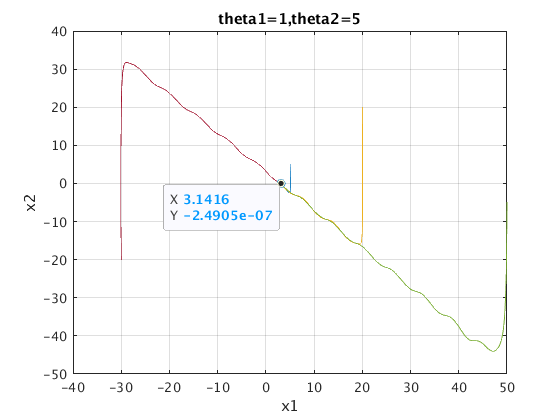
\includegraphics[width=14cm,keepaspectratio]{matlab/3_11/q_3_11_thetas_1_5.png}
\end{figure}\\

\pagebreak

$x_0=[20,20,20,20]:$\\

\begin{figure}[h]
  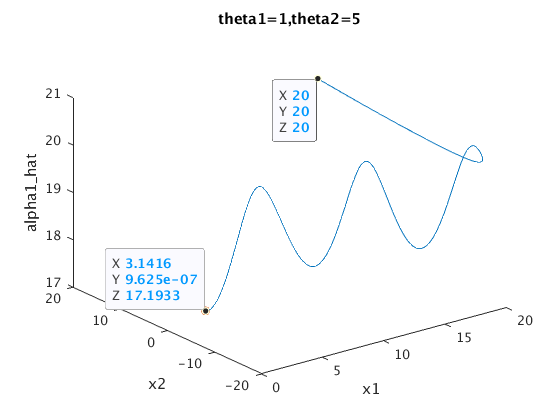
\includegraphics[width=9cm,keepaspectratio]{matlab/3_11/q_3_11_thetas_1_5_alpha1_convergence.png}
  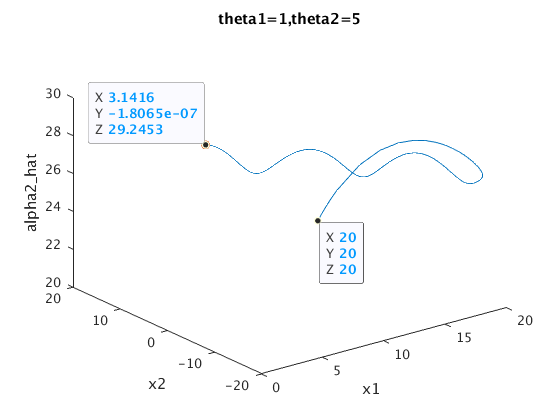
\includegraphics[width=9cm,keepaspectratio]{matlab/3_11/q_3_11_thetas_1_5_alpha2_convergence.png}
\end{figure}\\

From plots, $x_1 \to \pi ,x_2 \to 0, \hat{\alpha_1}-\alpha_1 \not \to 0, \hat{\alpha_2}-\alpha_2\not \to 0$\\

\end{itemize}

\end {document}
